%!TEX root=finmath2.tex

\chapter{Модель локальной волатильности}
\label{ch:locvol}
\chaptertoc

В модели локальной волатильности цена рискового актива задается уравнением $d S_t = r_tS_tdt + \sigma(t,S_t) S_t d W_t$, где функцию $\sigma(t,s)$ можно выбрать таким образом, что цены европейских опционов в модели будут совпадать с рыночными ценами, \te\ полностью исключить статическую ошибку.
В этой лекции мы докажем формулу Б.~Дюпира, которая дает выражения для $\sigma(t,s)$ через цены опционов.

\section{Формула Дюпира}
\subsection{Основной результат}

Пусть задана функция $\hat C(T,K)$, которая выражает рыночные цены опционов колл на конкретный базовый актив для всевозможных страйков $K>0$ и времен исполнения $T\in[0,T_{\max}]$.
Под рыночными ценами мы понимаем цены опционов, которые можно получить из биржевых данных%
\footnote{В реальности имеется конечный набор значений страйков и времен исполнения, \te\ функция $\hat C$ известна лишь в конечном числе точек.
Задача интерполяции цен опционов будет рассмотрена в разделе \ref{lv:s:ah}.}

Нашей целью будет построить модель, в который бы получались в точности такие же цены опционов.
Будем рассматривать процесс цены рискового актива вида
\begin{equation}
\label{lv:model}
d S_t = r_tS_t dt + \sigma(t,S_t) S_t d W_t,
\end{equation}
где $r_t$ "--- детерминированная процентная ставка (считается, что она известна и ограничена), а $\sigma(t,s)$ "--- неизвестная функция, которую нужно найти из условия совпадения цен опционов. 
Будем предполагать, что дивиденды в модели отсутствуют, но, тем не менее, все приводимые далее результаты останутся верными и для детерминированной ставки дивидендной доходности $q_t$ "--- нужно лишь в формулах заменить $r_t$ на $r_t-q_t$.

Считается, что исходная вероятностная мера $\P$ уже является мартингальной, поэтому коэффициент сноса равен безрисковой ставке (см.\ пояснение в разделе \ref{gen:s:na-prices} лекции \ref{ch:general}).
Пусть далее функция 
\[
C(T,K) = \frac1{B_T}\E(S_T-K)^+,
\]
где $B_T = e^{\int_0^T r_tdt}$, обозначает цены опционов колл в модели \eqref{lv:model}.

\begin{theorem}[\emph{формула Дюпира}]
\label{lv:t:dupire}
Пусть функция $\hat C(T,K)$ имеет непрерывные частные производные $\hat C'_T$, $\hat C'_K$, $\hat C''_{KK}$, причем $C'_T(T,K) + r_t K C'_K(T,K)\ge 0$ и $C''_{KK}(T,K)>0$  на $(0,T_{\max}]\times(0,\infty)$.
Для $t\in(0,T_{\max}]$, $s>0$ определим функцию
\begin{equation}
\label{lv:dupire}
\sigma(t,s) = \sqrt{\frac{2(\hat C'_T(t,s) + r_ts\hat C'_K(t,s))}{s^2\hat C''_{KK}(t,s)}}.
\end{equation}

Пусть для этой функции уравнение \eqref{lv:model} имеет слабое решение\footnote{Для $t=0$ определим $\sigma(t,s)$ произвольным образом, так, чтобы уравнение \eqref{lv:model} имело решение.}, являющееся строго положительным процессом, причем процесс $\tilde S_t = S_t/B_t$ является мартингалом и для каждого $t\in(0,T]$ величина $S_t$ имеет абсолютно непрерывное распределение.
Тогда $C(T,K) = \hat C(T,K)$ при всех $T\in[0,T_{\max}]$, $K>0$.
\end{theorem}

Итак, при выполнении условий теоремы существует функция $\sigma(t,s)$, с которой модель \eqref{lv:model} дает цены опционов, совпадающие с рыночными.
Такая функция $\sigma(t,s)$ называется \emph{локальной волатильностью}, построенной по данной поверхности цен $\hat C(T,K)$.
Само уравнение \eqref{lv:model} называется \emph{моделью локальной волатильности}.

\begin{remark}
Мы рассматриваем только цены опционов колл, потому что опционы пут в теории дают такую же локальную волатильность.
Действительно, в любой безарбитражной модели выполняется паритет цен опционов колл-пут, а также он выполняется в рыночных данных.
Следовательно, если модель воспроизводит рыночные цены опционов колл, то она воспроизводит и цены опционов пут.
\end{remark}

% \begin{remark}
% Бруно Дюпир получил формулу \eqref{lv:dupire} в работе \cite{Dupire94} без строгого обоснования. 
% Приводимое далее доказательство следует книге \cite{MusielaRutkowski09}.
% Оригинальное <<доказательство>> Б.~Дюпира приведено в разделе \ref{lv:s:dupire-proof}.
% \end{remark}


\subsection{Достоинства и недостатки модели локальной волатильности}
\label{lv:s:discussion}

Достоинство модели локальной волатильности заключается в точном воспроизведении рыночных цен ванильных опционов колл и пут в \emph{текущий} момент времени.
Как следствие, если какой-то производный инструмент можно реплицировать ванильными опционами, то модель локальной волатильности воспроизводит и его цену.

Недостатком модели является то, что она не гарантирует, что рыночные цены опционов будут равны модельным ценам в \emph{будущие} моменты времени,
что приводит к динамической ошибке репликации.
Более того, модель локальной волатильности может показывать динамику цен опционов качественно отличающуюся от того, как цены изменяются в реальности, причем эта динамика даже <<менее правильная>>, чем, скажем, в модели \bs.

Чтобы это увидеть, посмотрим, как изменяются улыбки подразумеваемой волатильности при изменении цены базового актива в модели локальной волатильности. Так как цены опционов однозначно определяются своими подразумеваемыми волатильностями, то о поведении цен опционов можно судить по поведению подразумеваемой волатильности, и наоборот.

Оказывается, что в модели локальной волатильности при изменении цены базового актива поверхность волатильности двигается в противоположном направлении, по сравнению с тем, как она обычно меняется в реальности.
На рис.~\ref{lv:f:iv-move} приведена иллюстрация этого факта на симулированных данных с помощью модели Хестона\footnote{Модель стохастической волатильности, которую мы будем изучать далее в курсе.}.
Синяя кривая представляет улыбку волатильности (\te\ функцию $K\mapsto\hat\sigma(T,K)$ для фиксированного $T$) в модели Хестона для некоторого набора параметров модели и цены базового актвиа $S_0=100$.
Зеленая кривая показывает, как в ней изменится улыбка волатильности, если цена базового актива вырастет на небольшое значение $\epsilon$, а все остальные параметры останутся неизменными.
Оранжевая кривая "--- это улыбка волатильности в модели локальной волатильности с функцией $\sigma(t,s)$ построенной по ценам опционов в исходной модели Хестона, после того как цена базового актива увеличится на $\epsilon$.
Видно, что в модели Хестона улыбка передвигается вправо, а в модели локальной волатильности влево и вниз\footnote{Более полное объяснение, почему так получается, приведено в разделе \ref{lv-s:s:hagan} дополнения \ref{ch:lv-s}.}.
На реальных рынках наблюдается динамика улыбок волатильности более похожая на ту, что в модели Хестона.

%%%%%%%%%%%%%%%%%%%%%%%%%%%%%%%%%%%%%%%%%%%%%%%%%
%%% Старый фрагмент
%%%%%%%%%%%%%%%%%%%%%%%%%%%%%%%%%%%%%%%%%%%%%%%%%
%Неверная динамика подразумеваемой волатильности означает неверную динамику цен опционов, а это приводит к динамической ошибке в модели, если использовать опционы для хеджирования других производных инструментов.

% При этом ее недостатком является жесткая связь между \emph{будущими} ценами опционов и ценой базового актива (эта связь возникает из-за того, что цена опциона однозначно определяется значением $S_t$ в силу марковского свойства модели).
% Как следствие, изменения поверхности подразумеваемой волатильности полностью определяются движением цены базового актива.

% Перечислим несколько причин, почему это является недостатком модели.
% Во-первых, в реальности волатильность зависит не только от того, какова в данный момент цена базового актива, но также и от того, как рынок пришел к ней.
% Можно провести мысленный эксперимент: если цена акции в текущий момент равна 100 и она <<равномерно>> росла на протяжении предыдущего года от значения 90, то волатильность будет на <<обычном>> уровне. Если же цена сначала выросла с 90 до 130, а потом резко упала до 100, то волатильность будет повышенной.

% Во-вторых, на величину волатильность могут оказывать влияние внешние источники случайности. Например, негативные экономические новости обычно приводят к повышенной волатильности.
%%%%%%%%%%%%%%%%%%%%%%%%%%%%%%%%%%%%%%%%%%%%%%%%%

\begin{figure}[h]
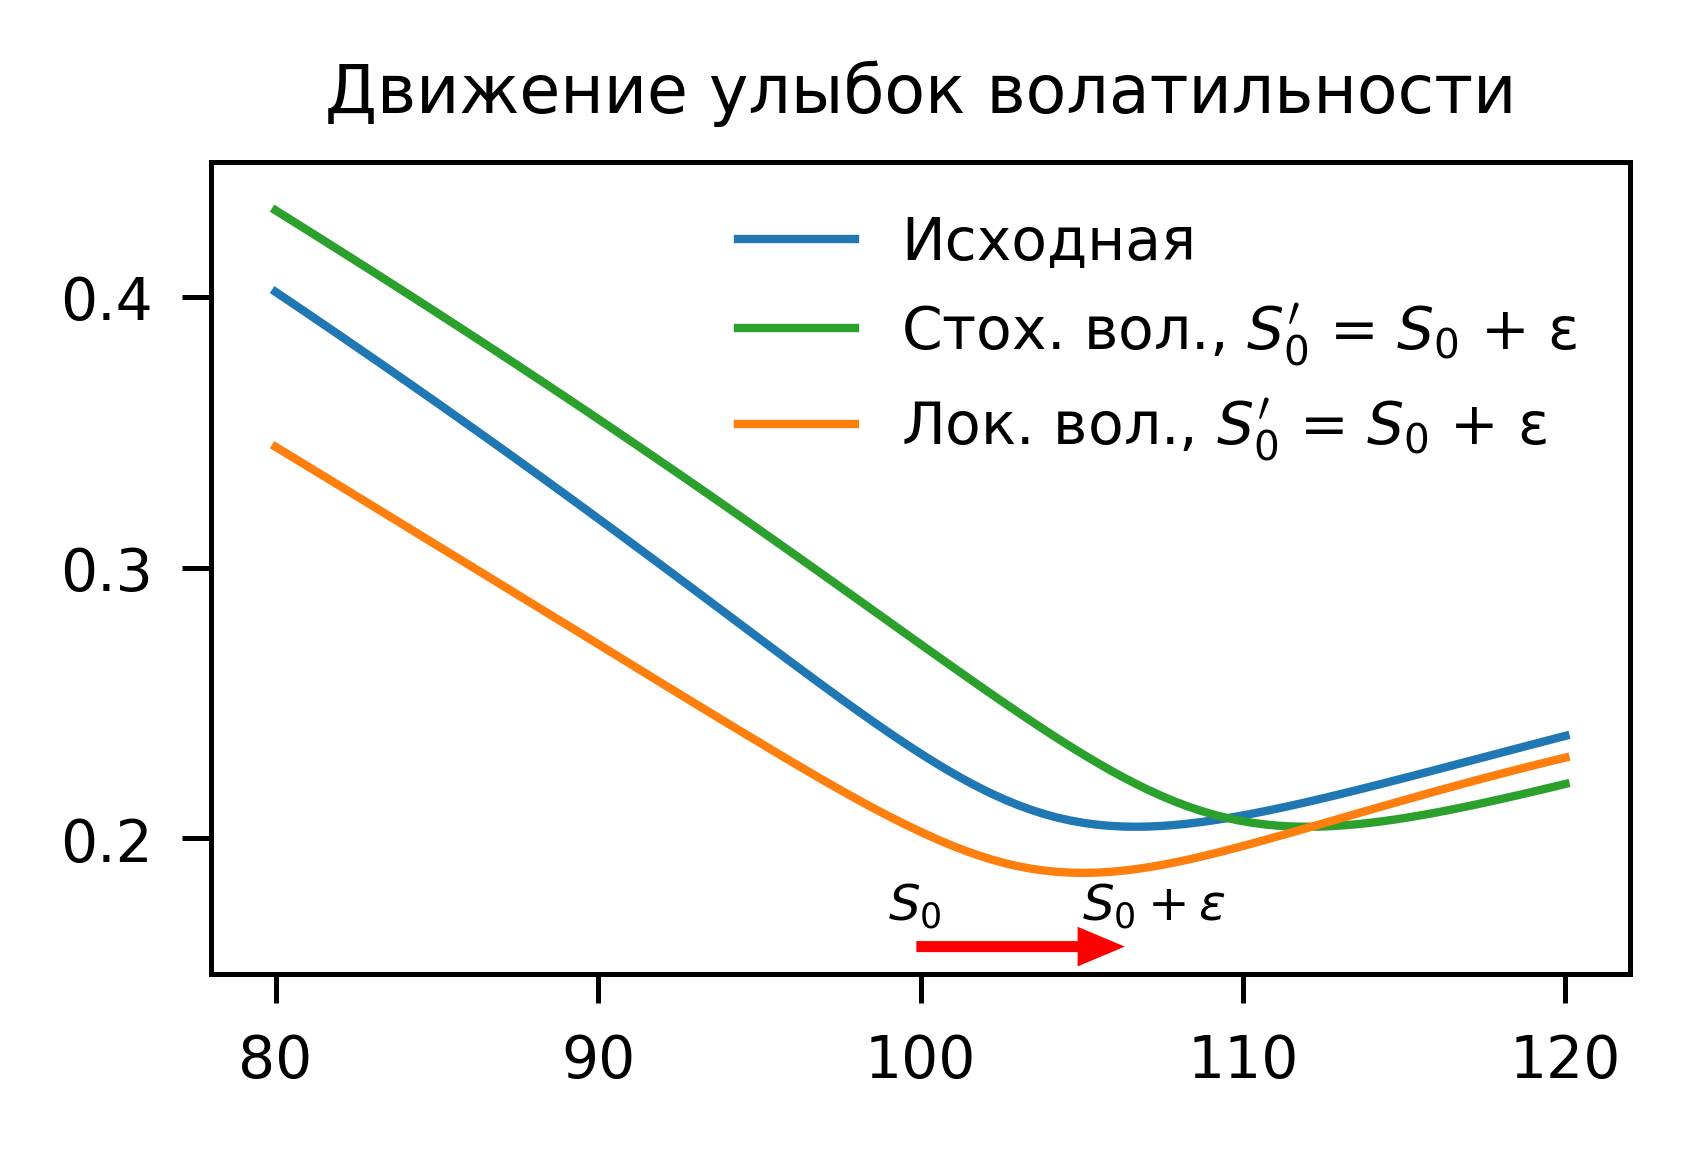
\includegraphics{pic/locvol-iv.png}
\centering
\caption{Изменение улыбок волатильности в модели локальной волатильности и модели стохастической волатильности при изменении цены базового актива.}
\label{lv:f:iv-move}
\end{figure}



\section{Вспомогательные результаты}
В этом разделе собраны технические результаты, которые потребуются для доказательства формулы Дюпира.
Приводимое доказательство следует книге \cite{MusielaRutkowski09}.
Оригинальное доказательство Б.~Дюпира приведено в разделе \ref{lv:s:dupire-proof}.

\subsection{Формула Бридена--Литценбергера}

Следующий результат в приложениях к оценке опционов впервые встречается в работе Д.~Бридена и Р.~Литценбергера \cite{BreedenLitzenberger78} и поэтому в литературе часто называется \emph{формулой Бридена"--~Литценбергера}.

\begin{proposition}
\label{1:l:bl}
Пусть $S\ge 0$ "--- случайная величина, $\E S<\infty$.
Обозначим $C(K) = \E(S-K)^+$, $K\in\R_+$.
Предположим, что $C\in C^2((0,\infty))$.
Тогда $S$ имеет абсолютно непрерывное распределение с плотностью $f(s)=C''(s)$.
\end{proposition}

\begin{proof}
Имеем $C(K) = \int_K^\infty (s-K) d F(s) = \int_K^\infty (K-s) d (1-F(s))$, где $F$ "--- функция распределения $S$.
Интегрируя по частям%
\footnote{Для интеграла Лебега"--~Стилтьеса справедлива следующая формула интегрирования по частям (см.~\cite{Shiryaev04}, гл.~II, \S\,6, теорема 11).
Пусть функции $F$, $G$ имеют ограниченную вариацию на отрезке $[a,b]$, причем $F$ непрерывна справа и имеет пределы слева в каждой точке, а $G$ непрерывна.
Тогда $F(b)G(b) - F(a)G(a) = \int_a^b F(x)d G(x) + \int_a^b G(x) d F(x)$.},
получаем
\[
C(K) = \lim_{b\to\infty} \left((K-b)(1-F(b)) + \int_K^b (1-F(s)) ds\right).
\]
Заметим, что $\lim\limits_{b\to\infty} b(1-F(b)) = 0$. Действительно, 
\[
0 = \lim\limits_{b\to\infty} \E S\I(S> b) \ge \lim_{b\to\infty} b \P(S> b) = \lim\limits_{b\to\infty} b(1-F(b)),
\]
где в первом равенстве воспользовались теоремой о мажорируемой сходимости и тем, что $\E S < \infty$.
Тогда $C(K) = \int_K^\infty (1-F(s)) ds$, откуда $C'(K) = F(K) - 1$.
Следовательно, $F(s)$ непрерывно дифференцируема и $f(s) = C''(s)$.
\end{proof}

\begin{remark}[смысл формулы Бридена"--~Литценбергера]
Пусть безрисковая процентная ставка равна 0.
Тогда, согласно формуле Бридена--Литценбергера, поверхность цен опционов колл $\hat C(T,K)$ задает семейство одномерных плотностей $f_t(s) = \hat C''_{KK}(t,s)$.
С другой стороны, цены опционов в модели $C(T,K) := \E(S_T-K)^+$ определяются одномерными распределениями величин $S_T$.
Таким образом, имеется взаимно-однозначное соответствие между ценами опционов колл (или пут) и одномерными распределениями процесса цены относительно эквивалентной мартингальной меры (при условии, что функция $C(T,K)$ и распределения величин $S_T$ достаточно хорошие). 
Рассуждение остается справедливым и в случае произвольной безрисковой ставки.

Как следствие, модель локальной волатильности можно рассматривать как модель, воспроизводящую заданные одномерные распределения процесса цены рискового актива. 
\end{remark}


\subsection{Локальное время}

Подробное изложение результатов о \emph{локальных временах} случайных процессов можно найти в книге \cite{RevuzYor}, гл.~VI; здесь же мы приведем без доказательств только нужные нам факты.

Далее в этом разделе $X$ "--- локальный мартингал вида%
\footnote{Все приводимые результаты остаются верными и для произвольных непрерывных локальных мартингалов, но в формулах нужно будет заменить $\sigma_t^2 dt$ на $d\qc X_t$, где $\qc X_t$ "--- \emph{квадратическая характеристика} непрерывного локального мартингала $X$, \te\  неубывающий непрерывный согласованный процесс такой, что $X_t^2 - \qc X_t$ является локальным мартингалом.}
$d X_t = \sigma_t d W_t$.

\begin{proposition}[\emph{формула Танаки}, \cite{RevuzYor}, гл.~VI, теоремы 1.2 и 1.7]
Для любого $a\in \R$ существует \as-единственный неубывающий непрерывный согласованный процесс $L_t^a(X)$ такой, что 
\[
|X_t - a| = |X_0-a| + \int_0^t \sgn(X_s-a) d X_s + L_t^a(X),
\]
где $\sgn(x) = 1$ для $x\ge 0$ и $\sgn(x)=-1$ для $x< 0$ (так, что правая производная $|x|' = \sgn(x))$.

Более того, существует модификация процесса $L_t^a(X)$, которая непрерывна по паре переменных $(t,a)$.
\end{proposition}

\begin{definition}
Процесс $L_t^a(X)$ называется \emph{локальным временем} процесса $X$ на уровне $a$.
\end{definition}

Далее всегда будем рассматривать модификацию локального времени, которая непрерывна по паре переменных.

\begin{remark}
Формула Танаки обобщает формулу Ито на негладкую функцию $f(x) = |x-a|$. 
По формуле Ито $|X_t - a| = |X_0-a| + \int_0^t \sgn(X_s-a) d X_s + \int_0^t f''(X_s) \sigma_s^2 ds$, однако производная $f''$ не определена.
Формула Танаки говорит, что вместо $\int_0^t f''(X_s) \sigma_s^2 ds$ нужно поставить локальное время.
\end{remark}


\medskip
Напомним, что если функция $f$ выпукла на $\R$, то у нее в каждой точке существует левая и правая производная; левая производная непрерывна слева, а правая справа, причем обе производные не убывают.
В частности, из этих свойств следует, что для выпуклой функции можно определить $\sigma$-конечную меру на $\R$ по формуле $\mu_f((a,b]) = f'(b) - f'(a)$, где $f'$ "--- правая производная.
Далее будем обозначать ее как $f''(da)$.

\begin{proposition}[\emph{формула Ито--Танаки--Мейера}, \cite{RevuzYor}, гл.~VI, теорема 1.5]
Если функция $f(x)$ выпукла, то 
\[
f(X_t) = f(X_0) + \int_0^t f'_-(X_s) dX_s + \frac12 \int_\R L_t^a(X) f''(da).
\]
\end{proposition}

\begin{example}
Если $f(x) = (x-a)^+$, то правая производная $f'(x) = \I(x\ge a)$. Тогда
\[
(X_t-a)^+ = (X_0-a)^+ + \int_0^t \I(X_t\ge a) dX_t + \frac12 L_t^a(X).
\]
\end{example}

\begin{proposition}
\label{lv:l:martingale}
Пусть локальный мартингал $X_t$ вида $dX_t = \sigma_t dW_t$ является настоящим мартингалом.
Тогда для любого $a\in\R$ процесс $Y_t = \int_0^t \I(X_t\ge) d X_t$ тоже является мартингалом. 
Как следствие, справедливо равенство
\[
\frac12\E L_t^a(X) = \E(X_t-a)^+ - (X_0-a)^+.
\] 
\end{proposition}

% \begin{proof}
% По неравенству Йенсена процесс $(X_t-a)^+$ является субмартингалом.
% Из \emph{разложения Дуба"--~Мейера}%
% \footnote{Любой субмартингал $S_t$ представим в виде $S_t = S_0 + M_t + A_t$, где $M_t$ "--- локальный мартингал, $A_t$ "--- процесс ограниченной вариации, $M_0=A_0=0$, причем процессы $M_t$ и $A_t$ единственны \as{}}
%  следует, что его можно представить в виде $(X_t-a)^+ = (X_t-a)^+ + M_t + A_t$, где $M_t$ "--- непрерывный локальный мартингал, $A_t$ "--- непрерывный неубывающий согласованный процесс, $M_0=A_0=0$. 
% По формуле Ито"--~Танаки"--~Мейера имеем $(X_t-a)^+ = (X_0-a)^+ + \int_0^t \I(X_t>a) d X_t + \frac12 L_t^a(X)$, и следовательно
% \[
% M_t - \int_0^t \I(X_t>a) d X_t = \frac12 L_t^a(X) - A_t.
% \]
% Левая часть является непрерывным локальным мартингалом, а правая "--- непрерывным процессом ограниченной вариации. Из единственности в разложении Дуба"--~Мейера следует, что они обе нулевые. Таким образом, $\int_0^t \I(X_t>a) d X_t = M_t$ "--- мартингал.
% \end{proof}

% \begin{proof}
% По формуле Ито"--~Танаки"--~Мейера имеем $(X_t-a)^+ = (X_0-a)^+ + \int_0^t \I(X_t>a) d X_t + \frac12 L_t^a(X)$.
% Вычисляя математическое ожидание от обеих частей и применяя лемму \ref{lv:l:martingale}, получаем доказываемое утверждение.
% \end{proof}

Короткое доказательство предложения \ref{lv:l:martingale} для более общего случая можно найти в статье \cite{HamzaKlebaner22}. 


\begin{proposition}[формула для времени пребывания, \cite{RevuzYor}, гл.~VI, теорема 1.6]
Для любой неотрицательной измеримой функции $f(x)$ выполнено равенство
\[
\int_\R f(a) L_t^a(X) da = \int_0^t f(X_s) \sigma_s^2 ds.
\]  
\end{proposition}

\begin{remark}
Поясним, откуда возникает формула для времени пребывания.
Можно дать эквивалентное определение локального времени:
\[
L_t^a(X) = \lim_{\epsilon\downarrow 0} \frac{1}{2\epsilon} \int_0^t \I(|X_s-a|< \epsilon) \sigma^2_s ds.
\]
По своему смыслу эта формула означает, что локальное время является плотностью \emph{меры времени пребывания в точке $a$} (см.~\cite{RevuzYor}, гл.~VI, следствие 1.9), где мера пребывания $\mu$ "--- это случайная мера 
\[
\mu_t(\omega, A) = \int_0^t \I(X_s \in A) ds,
\] 
для борелевских множеств $A$.
Если приближать измеримую функцию $f$ простыми функциями (линейными комбинациям индикаторов), то из этого определения и получается формула времени пребывания.
\end{remark}


\section{Доказательство формулы Дюпира}
\subsection{Случай нулевой процентной ставки}

Пусть сначала $r_t\equiv 0$.
Согласно предложению \ref{lv:l:martingale}, 
\[
C(T,K) = (S_0-K)^+ + \frac 12 \E L_T^K(S).
\]
Обозначим $f(t,s)$ плотность величины $S_t$.
Тогда, умножая обе части полученного равенства на произвольную гладкую функцию $h(s)$ с компактным носителем и интегрируя, получаем
\begin{multline*}
\int_\R h(K) C(T,K) dK 
= \int_\R h(K)(S_0-K)^+  dK + \frac12 \E \int_0^T h(S_t) \sigma^2(t,S_t) S_t^2 dt \\
=\int_\R h(K)(S_0-K)^+  dK + \frac12 \int_0^T \int_\R h(K)f(t,K) \sigma^2(t,K)K^2 dK dt \\
= \int_\R h(K) 
  \biggl(
    (S_0-K)^+ + \frac12\int_0^T C''_{KK}(t,K) \sigma^2(t,K)K^2 dt
  \biggr) dK,
\end{multline*}
где в первом равенстве воспользовались формулой времени пребывания, во втором представили математическое ожидание в виде интеграла по плотности и поменяли пределы интегрирования, а в третьем равенстве воспользовались формулой Бридена"--~Литценбергера.
В силу произвольности функции $h$ из совпадения интегралов получаем равенство подынтегральных функций
\[
C(T,K) = (S_0-K)^+ + \frac12 \int_0^T C''_{KK}(t,K) \sigma^2(t,K) K^2dt.
\]
Дифференцируя по $T$, получаем доказываемое утверждение.

\subsection{Общий случай}
\label{lv:ss:general-case}
Покажем как случай произвольной детерминированной процентной ставки $r_t$ можно свести к $r_t\equiv 0$.
Для заданной функции $C(T,K)$ и функции $\sigma(t,s)$, определяемой по формуле Дюпира \eqref{lv:dupire}, введем две новые функции
\[
\hat C^*(T,K) = \hat C(T,KB_T), \qquad 
\sigma^*(t,s) = \sigma(t, sB_t).
\]
Непосредственно проверяется, что
\[
\sigma^*(t,s) = \sqrt{\frac{2(\hat C^*)'_T(t,s)}{s^2(\hat C^*)''_{KK}(t,s)}}.
\]
Кроме того, используя формулу Ито, находим, что, если процесс $S_t$ удовлетворяет уравнению \eqref{lv:model} с функцией $\sigma(t,s)$, то дисконтированная цена $S_t^* = S_t/B_t$ удовлетворяет уравнению $d S_t^* = \sigma^*(t,S_t^*) S_t^* d W_t$.

Таким образом, к функциям $\hat C^*$, $\sigma^*$ и процессу $S_t^*$ можно применить доказываемую теорему в случае $r_t\equiv 0$, откуда следует, что цены опционов $C^*(T,K) = \E(S_T^*-K)^+$  удовлетворяют равенству $C^*(T,K)=\hat C^*(T,K)$. 

Остается заметить, что $C(T,KB_T) = B_T^{-1} \E(S_T-KB_T)^+ = \E(S_T^* - K)^+ = C^*(T,K)$, и, следовательно, $C(T,KB_T) = \hat C(T,KB_T)$.
Тогда $C(T,K) = \hat C(T,K)$.


\subsection{Другое доказательство}
\label{lv:s:dupire-proof}

Приводимая далее цепочка равенств следуют рассуждениям в статье \cite{Dupire94}.
Некоторые переходы в ней трудно обосновать строго, поэтому ее нельзя назвать формальным доказательством.

Рассмотрим только случай $r_t\equiv 0$.
Пусть $f(t,s)$ "--- плотность $S_t$.
Тогда
\[
\begin{split}
C'_T(T,K) 
&= \int_K^\infty (s-K) \prt ft(T,s) ds 
  = \text{[прямое уравнение Колмогорова]} \\[1em] 
&= \frac12 \int_K^\infty (s-K)\prtt{}{s}(\sigma^2 s^2 f)(T,s) ds 
  = \text{[интегрирование по частям]}\\[1em] 
&= -\frac12\int_K^\infty \prt{}s (\sigma^2y^2f)(T,s) ds \\[1em]
&= \frac12 \sigma^2(T,K)K^2 f(T,K)
  = \text{[формула Бридена--Литценбергера]}\\[1em]
&= \frac12 \sigma^2(T,K) K^2 C''_{KK}(T,K).
\end{split}
\]
Получаем, что если $C(T,K)$ "--- цены опционов колл в модели, то функция $\sigma(t,s)$ должна удовлетворять равенству $\sigma^2(t,s) = 2C'_T(t,s)/C''_{KK}(t,s)$.
Соответственное, если модель воспроизводит рыночные цены опционов ($C=\hat C$), то верна формула Дюпира \eqref{lv:dupire}.


\section{Алгоритм Андреасена"--~Хьюджа}
\label{lv:s:ah}
\subsection{Построение локальной волатильности по дискретным ценам опционов}
Пусть задан конечный набор времен исполнения $T_1<T_2<\ldots<T_m$ и для каждого времени исполнения задан набор цен опционов колл $\hat C_{i,j}=\hat C(T_i, \hat K_{i,j})$, где $\hat K_{i,1} < \ldots < \hat K_{i,n_i}$ "--- различные страйки.
В этом разделе мы приведем алгоритм Андреасена"--~Хьюджа \cite{AndreasenHuge10} построения функции локальной волатильности $\sigma(t,s)$ по ценам $\hat C_{i,j}$.

Далее будем считать безрисковую ставку равной 0.
В случае ненулевой ставки можно построить локальную волатильность $\sigma^*(t,s)$ для дисконтированного процесса цены (для этого нужно применить тот же самый алгоритм, но считая, что вместо страйков $\hat K_{i,j}$ заданы страйки $\hat K_{i,j} B_{T_i}$, а цены опционов те же "--- это следует из рассуждений в доказательстве формулы Дюпира, см.~раздел \ref{lv:ss:general-case}), и тогда искомая локальная волатильность будет $\sigma(t,s) = \sigma^*(t,s/B_t)$. 

Положим $T_0=0$.
Функция $\sigma(t,s)$ будет кусочно-постоянной по $t$ на промежутках $(T_{i-1}, T_i]$ и кусочно-линейной по $s$ на промежутках $(\hat K_{i,j-1}, \hat K_{i,j}]$, а именно для $t\in (T_{i-1}, T_i]$ положим
\[
\sigma(t, s) = \begin{cases}
a_{i,1}, 
  &\text{при } s\le \hat K_{i,1},\\
\dfrac{a_{i,j-1}(s-\hat K_{i,j-1}) + a_{i,j}(\hat K{i,j} - s)}{\hat K_{i,j}-\hat K_{i,j-1}}, 
  &\text{при } \hat K_{i,j-1}< s \le \hat K_{i,j},\\
a_{i,n_i}, 
  &\text{при } s> \hat K_{i,n_i},
\end{cases}
\]
где значения $a_{i,j}$ предстоит найти.
Идея состоит в том, что по значениям $a_{i,j}$ можно вычислить цены опционов $C(T, K)$ в модели, и, следоватлеьно, нужно выбрать $a_{i,j}$ так, чтобы получаемые цены в точках $(T_i, K_{i_j})$ были как можно ближе к заданным значениям $\hat C_{i,j}$.

Покажем, как по выбранным $a_{i,j}$ найти цены опционов в модели.
Будем искать функцию $C(T,K)$ для $T=T_i$ по индукции. Для $i=0$ положим $C(0, K) = (S_0-K)^+$.
Далее воспользуемся тем, что формулу Дюпира можно записать в виде
\[
C'_T(T,K) = \frac12 K^2 \sigma^2(T,K)C''_{KK}(T,K).
\]
Если функция $C(T_{i-1}, K)$ построена, то, дискретизируя производную по $T$, получаем дифференциальное уравнение на функцию $C(T_i,K)$:
\[
\frac{C(T_{i},K) - C(T_{i-1},K)}{\Delta T_i} = \frac12 K^2 \sigma^2(T_i,K)C''_{KK}(T_i,K),
\]
где $\Delta T_i = T_i - T_{i-1}$.
Чтобы его решить, воспользуемся методом конечных разностей и дискретизируем производную по $K$.
Для этого зафиксируем набор страйков $K_0,\dots,K_m$, где $K_l = K_0 + l\Delta K$, так что $K_0$ достаточно мало, а $K_m$ достаточно велико.
Будем использовать один и тот же набор $K_l$ для всех значений $T_i$, поэтому промежуток $(K_0, K_m)$ должен, как минимум, покрывать все страйки $\hat K_{i,j}$, для которых нам даны цены $\hat C_{i,j}$.

Для $l=1,\dots,m-1$ получаем разностные уравнения
\begin{multline}
\label{lv:ah-system}
\frac{C(T_i,K_l) - C(T_{i-1}, K_l)}{\Delta T_i} \\
= \frac12 K_l^2 \sigma^2(T_i,K_l) \frac{C(T_i,K_{l-1}) -2C(T_i,K_l) + C(T_i,K_{l+1})}{(\Delta K)^2}.
\end{multline}
Для $l=0$ и $l=m$ добавим условия $C''_{KK}(T_i,K_l) = 0$, что даст уравнения
\begin{gather}
\label{lv:ah-boundary-1}
C(T_i,K_0) - C(T_{i-1}, K_0) = 0,\\
\label{lv:ah-boundary-2}
C(T_i,K_m) - C(T_{i-1}, K_m) = 0.
\end{gather}

Систему линейных уравнений \eqref{lv:ah-system}--\eqref{lv:ah-boundary-2} можно представить в матричном виде $A c_i = c_{i-1}$, где $c_i=(c_{i,0},\dots,c_{i,l})$ "--- вектор неизвестных, соответствующих значениям $C(T_i,K_l)$, а матрица $A$ имеет трехдиагональный вид
\[
A = \begin{pmatrix}
1 & 0 \\
-z_1 &1+2z_1 & -z_1\\
& -z_2 &1+2z_2 & -z_2\\
& & \ddots & \ddots & \ddots \\
& & & -z_{m-1} &1+2z_{m-1} & -z_{m-1}\\
& & & & 0 & 1
\end{pmatrix},
\]
где
\[
z_l = \frac{\Delta T_i}{2(\Delta K)^2} K_l^2\sigma^2(T_i,K_l).
\]
Матрица $A$ обладает свойтвом строгого диагонального преобладания (каждый элемент на главной диагонали по модулю больше суммы модулей других элементов в строке), и хорошо известно, что такие матрицы обратимы.
Следовательно, рассматриваемая система уравнений имеет единственное решение.
Трехдиагональный вид позволяет эффективно находить его численно, например, \emph{методом прогонки}.

Пусть $c_i(a_i)$ обозначает решение этой системы, зависящее от вектора параметров $a_i=(a_{i,1},\dots,a_{i,n_i})$. 
Тогда для выбора $a_i$ решается оптимизационная задача
\[
\sum_{j=1}^{n_i} (\hat C_{i,j} - c_{i,j}(a_i))^2 \to \text{min}.
\]
После нахождения $a_i$ переходят к аналогичной процедуре для нахождения $a_{i+1}$, и так далее.


\subsection{Интерполяция цен опционов}
Алгоритм Андреасена"--~Хьюджа также используется для интерполяции цен опционов, \te\ нахождения $\hat C(T,K)$ в точках, отличных от $(T_i,K_{i,j})$.

Пусть $T\in(T_{i-1},T_i)$ (или $T>T_m$ "--- для задачи экстраполяции).
Тогда значения $C(T,K_l)$ находятся из решения системы \eqref{lv:ah-system}--\eqref{lv:ah-boundary-2} с $T$ вместо $T_i$, \te\ решая $Ac = c_{i-1}$, где $c$ "--- вектор неизвестны цен $C(T,K_l)$, а матрица $A$ имеет такой же вид, как и выше, но с элементами
\[
z_l = \frac{T-T_{i-1}}{2(\Delta K)^2} K_l^2\sigma^2(T_i,K_l).
\]
После нахождения $C(T,K_l)$ цены в промежуточных точках $K\in (K_0,K_m)$ можно получить линейной интерполяцией, а для $K< K_0$ или $K>K_m$ экстраполировать цены в виде $C(T,K) = (S_0-K)^+$ (это соответствует тому, что выше мы считали $C''_{KK}(T_i,K_0) = C''_{KK}(T_i,K_m) = 0$, что вместе с начальным условием $C(0,K) = (S_0-K)^+$  по формуле Дюпира дает равенство $C(T_i,K_l) = C(T_i,K_l) = (S_0-K_l)^+$ для $l=0,m$.)



% Достоинство модели локальной волатильности заключается в том, что она дает правильные (\te\ равные рыночным) цены опционов колл и пут в текущий момент времени.
% Как следствие, она дает правильные цены всех деривативов, которые могут быть реплицированы \emph{статическим портфелем} из безрискового актива, рискового актива и опционов, \te\ таким портфелем, который покупается в момент $t=0$ и не ребалансируется до момента экспирации дериватива
% \footnote{Например, так можно реплицировать любую выплату вида $X=f(S_T)$ при условии, что функция $f$ <<не слишком плохая>>.}.
% Если статическая репликация дериватива невозможна, то приходится делать \emph{динамическую репликацию}, \te\ использовать торговую стратегию, портфель которой изменяется со временем.
% Если такой динамический портфель включает опционы, то важно, чтобы движение их цен, предсказываемое моделью, соответствовало тому, как они движутся в реальности.

% Одним из недостатков модели локальной волатильности является то, что она предсказывает неверное движение улыбок волатильности\footnote{Напомним, что \emph{улыбкой волатильности} называется функция $K\mapsto \hat\sigma(T,K)$ при фиксированном $T$, где $\hat\sigma$ "--- подразумеваемая волатильность.} и, следовательно, неверное движение цен опционов.
% Чтобы это показать, мы получим приближенную формулу, выражающую подразумеваемую волатильность через локальную, которая интересна и сама по себе.

% Будем рассматривать модель локальной волатильности, в которой волатильность не зависит от времени, \te\ цена рискового актива удовлетворяет уравнению
% \begin{equation}
% \label{lv:time-indep}
% dS_t = r_tS_t dt + \sigma(S_t) S_t dW_t,
% \end{equation}
% причем будем считать, что у этого уравнения имеется единственное слабое решение такое, что дисконтированная цена $\tilde S_t$ является мартингалом.

% Пусть $\hat\sigma(T, s, K)$ обозначает подразумеваемую волатильность опциона колл или пут с временем до исполнения $T$, страйком $K$ при текущей цене базового актива $s$.

% \begin{lemma}
% В модели \ref{lv:time-indep} выполнено равенство
% \[
% C(\tau, s, K) = C(\tau, K, s)
% \]
% \end{lemma}

% \begin{proof}
% Определим процесс $Z_t = \tilde S_t/S_0$.
% В силу условий на процесс цены, $Z_t$ является положительным  мартингалом с $\E Z_t = 1$.
% Следовательно, можно определить вероятностную меру $\Q = Z_Td\P$, эквивалентную $\P$.

% Так как 
% \[
% Z = \exp(\int_0^T \sigma(S_t)dW_t - \frac12\int_0^T\sigma^2(S_t)dt,
% \]
% то по теореме Гирсанова процесс
% \[
% \tilde W_t = W_t - \int_0^t \sigma(S_u)du
% \]
% является броуновским движением относительно $\Q$. 
% Кроме того, заметим, что 
% При этом заметим, что 
% \[
% \frac{1}{Z_t} =  \exp(-\int_0^t \sigma(S_u)dW_u + \frac12\int_0^t\sigma^2(S_u)dt) = 
% \exp(\int_0^t \sigma(S_u)d \tilde W_t - \frac12\int_0^t\sigma^2(S_u)dt).
% \]
% Таким образом, 
% Тогда имеем
% \begin{multline*}
% C(T,S_0,K) = B_T^{-1} \E(S_T - K)^+ = B_T^{-1} \E Z_T (S_0 - \frac{K}{Z_T})^+
% \end{multline*}
%\end{proof}







% Прежде чем переходить к доказательству, поясним, как из формулы \eqref{lv:hw} качественно увидеть характер изменения улыбки волатильности при изменении цены базового актива. 
% Пусть $\hat\sigma_0(T,K)$ обозначает улыбку волатильности для фиксированной экспирации $T$ в момент времени $t=0$.
% Если рассматривать страйки $K$ вблизи значения $S_0$, то в формуле \eqref{lv:hw} можно ограничиться только первым членом в правой части (вклад второго будет мал). 
% Тогда получаем, что
% \[
% A(s) \approx  \hat\sigma_0(T, 2 s - S_0) s.
% \]
% Если цена $S_0$ изменится на $\epsilon$ за время $\Delta t$, то новая улыбка волатильности станет равна
% \[
% \hat\sigma_{\Delta t}(T, K) 
% \approx \frac{A((S_0+ \epsilon + K)/2)}{(S_0+\epsilon+K)/2}
% \approx \hat\sigma_0(T, K + \epsilon).
% \]
% Следовательно, если $\epsilon>0$, то улыбка сдвигается влево, а если $\epsilon<0$, то вправо (см.~рис.~\ref{lv:f:smile}).
% В реальности наблюдается противоположная динамика: улыбка имеет тенденцию двигаться в том же направлении, что и цена базового актива.

% Так как имеется однозначное соответствие между подразумеваемыми волатильностями и ценами ванильных опционов, то данное обстоятельство означает, что модель локальной волатильности приводит к неверной динамике цен опционов. 
% Как следствие, это приводит к ошибкам в хеджировании, если хеджирующий портфель содержит опционы. 

% \medskip
% \begin{figure}
% \centering
% \begin{tikzpicture}
% \draw (1,0) -- (3,0);
% \draw[->] (4,0)--(5.5,0)  node[below] {\footnotesize $K$};
% \draw plot [smooth] coordinates {(2,2.5) (3,0.5) (4.5,2.5)} 
%   node[right] {\footnotesize $\hat\sigma_0$};
% \draw[dashed] plot [smooth] coordinates {(1,2.5) (2,0.5) (3.5,2.5)}
%   node[right] {\footnotesize $\hat\sigma_{\Delta t}$};
% \draw (3,0) node[below] {\footnotesize $S_0$};
% \draw (4,0) node[below,xshift=5mm] {\footnotesize $S_0+\epsilon$};
% \draw[blue,thick] (3,0.05)--(3,-0.05);
% \draw[blue,thick,->] (3,0) -- (4,0);
% \draw[red,thick,->] (2.18,2) -- (1.18,2);
% \end{tikzpicture}
% \caption{Движение улыбки волатильности при изменении цены базового актива.}
% \label{lv:f:smile}
% \end{figure}


\summary
\begin{itemize}
\item Модель локальной волатильности: $d S_t = r_tS_t dt + \sigma(t,S_t)S_t d W_t$, где функцию $\sigma(t,s)$ нужно выбрать так, что модель будет в точности воспроизводить рыночные цены опционов колл (и, следовательно, цены опционов пут).

\item Формула Дюпира дает явное выражение для функции $\sigma(t,s)$ через поверхность рыночных цен опционов колл $\hat C(T,K)$:
\[
\sigma(t,s) = \sqrt{\frac{2(\hat C'_T(t,s) + r_ts\hat C'_K(t,s))}{s^2\hat C''_{KK}(t,s)}}.
\]

\item Достоинство модели локальной волатильности: точное воспроизведение цен опционов и подразумеваемых волатильности.
Недостаткок: неверная динамика цен опционов и подразумеваемой волатильности.

\item Алгоритм Андреасена"--~Хьюджа позволяет построить локальную волатильность по дискретному набору цен опционов, а также интерполировать и экстраполировать цены опционов на значения времени исполнения и страйка, отсутствующие в рыночных данных.
\end{itemize}
